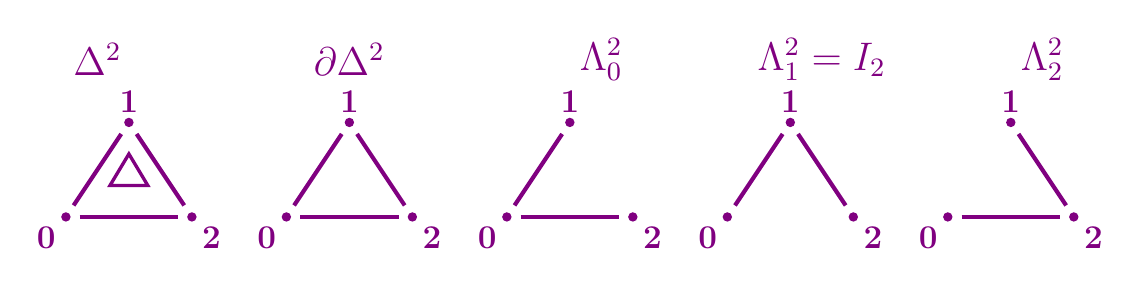
\begin{tikzpicture}[
    scale=0.8,
    thick,
    color=violet, % Match the ink color
    % Define the style for the vertices (small filled dots)
    dot/.style={circle, fill=violet, inner sep=1.2pt, outer sep=0pt},
    % Define the style for edges (gap near vertices, thick lines)
    edge/.style={line width=1.5pt, shorten <=5pt, shorten >=5pt},
    % Font settings
    font=\large\bfseries
]

    % --- Figure 1: Delta^2 (Filled Triangle) ---
    \begin{scope}[shift={(0,0)}]
        % Coordinates
        \coordinate (v0) at (0,0);
        \coordinate (v1) at (1,1.5);
        \coordinate (v2) at (2,0);
        
        % Main Label
        \node[scale=1.2] at (0.5, 2.5) {$\Delta^2$};
        
        % Edges
        \draw[edge] (v0) -- (v1);
        \draw[edge] (v1) -- (v2);
        \draw[edge] (v0) -- (v2);
        
        % Inner Triangle decoration
        \draw[line width=1.2pt] (0.7, 0.5) -- (1, 1.0) -- (1.3, 0.5) -- cycle;

        % Vertices and Labels
        \node[dot] at (v0) {}; \node[text=violet, below left] at (v0) {0};
        \node[dot] at (v1) {}; \node[text=violet, above]      at (v1) {1};
        \node[dot] at (v2) {}; \node[text=violet, below right] at (v2) {2};
    \end{scope}


    % --- Figure 2: Boundary of Delta^2 ---
    \begin{scope}[shift={(3.5,0)}]
        \coordinate (v0) at (0,0);
        \coordinate (v1) at (1,1.5);
        \coordinate (v2) at (2,0);
        
        \node[scale=1.2] at (1, 2.5) {$\partial \Delta^2$};
        
        % Edges (Hollow)
        \draw[edge] (v0) -- (v1);
        \draw[edge] (v1) -- (v2);
        \draw[edge] (v0) -- (v2);
        
        \node[dot] at (v0) {}; \node[text=violet, below left] at (v0) {0};
        \node[dot] at (v1) {}; \node[text=violet, above]      at (v1) {1};
        \node[dot] at (v2) {}; \node[text=violet, below right] at (v2) {2};
    \end{scope}


    % --- Figure 3: Lambda^2_0 (Horn 0) ---
    \begin{scope}[shift={(7,0)}]
        \coordinate (v0) at (0,0);
        \coordinate (v1) at (1,1.5);
        \coordinate (v2) at (2,0);
        
        \node[scale=1.2] at (1.5, 2.5) {$\Lambda^2_0$};
        
        % Edges (Missing face opposite 0, i.e., missing 1-2)
        \draw[edge] (v0) -- (v1);
        \draw[edge] (v0) -- (v2);
        
        \node[dot] at (v0) {}; \node[text=violet, below left] at (v0) {0};
        \node[dot] at (v1) {}; \node[text=violet, above]      at (v1) {1};
        \node[dot] at (v2) {}; \node[text=violet, below right] at (v2) {2};
    \end{scope}


    % --- Figure 4: Lambda^2_1 = I_2 (Horn 1) ---
    \begin{scope}[shift={(10.5,0)}]
        \coordinate (v0) at (0,0);
        \coordinate (v1) at (1,1.5);
        \coordinate (v2) at (2,0);
        
        \node[scale=1.2] at (1.5, 2.5) {$\Lambda^2_1 = I_2$};
        
        % Edges (Missing face opposite 1, i.e., missing 0-2)
        \draw[edge] (v0) -- (v1);
        \draw[edge] (v1) -- (v2);
        
        \node[dot] at (v0) {}; \node[text=violet, below left] at (v0) {0};
        \node[dot] at (v1) {}; \node[text=violet, above]      at (v1) {1};
        \node[dot] at (v2) {}; \node[text=violet, below right] at (v2) {2};
    \end{scope}


    % --- Figure 5: Lambda^2_2 (Horn 2) ---
    \begin{scope}[shift={(14,0)}]
        \coordinate (v0) at (0,0);
        \coordinate (v1) at (1,1.5);
        \coordinate (v2) at (2,0);
        
        \node[scale=1.2] at (1.5, 2.5) {$\Lambda^2_2$};
        
        % Edges (Missing face opposite 2, i.e., missing 0-1)
        \draw[edge] (v1) -- (v2);
        \draw[edge] (v0) -- (v2);
        
        \node[dot] at (v0) {}; \node[text=violet, below left] at (v0) {0};
        \node[dot] at (v1) {}; \node[text=violet, above]      at (v1) {1};
        \node[dot] at (v2) {}; \node[text=violet, below right] at (v2) {2};
    \end{scope}

\end{tikzpicture}

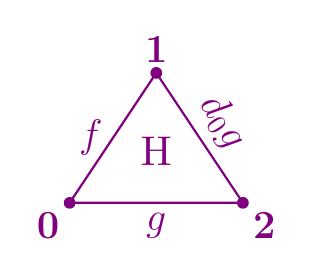
\begin{tikzpicture}[
    scale=1.1, 
    thick, 
    color=violet, 
    every node/.style={text=violet},
    dot/.style={circle, fill=violet, inner sep=1.5pt, outer sep=0pt}
]

    % Define coordinates
    \coordinate (O) at (0,0);       % Vertex 0
    \coordinate (A) at (1, 1.5);    % Vertex 1
    \coordinate (B) at (2, 0);      % Vertex 2

    % Draw the triangle and edge labels
    \draw (O) -- node[left] {\Large $f$} (A) 
              -- node[sloped, above] {\Large $d_0 g$} (B) 
              -- node[below] {\Large $g$} cycle;

    % Draw vertices (dots)
    \node[dot] at (O) {};
    \node[dot] at (A) {};
    \node[dot] at (B) {};

    % Draw vertex labels (0, 1, 2)
    \node[below left, text=violet] at (O) {\Large \bfseries 0};
    \node[above, text=violet] at (A) {\Large \bfseries 1};
    \node[below right, text=violet] at (B) {\Large \bfseries 2};

    % Draw center label H
    \node[scale=1.5] at (1, 0.6) {H};

\end{tikzpicture}


            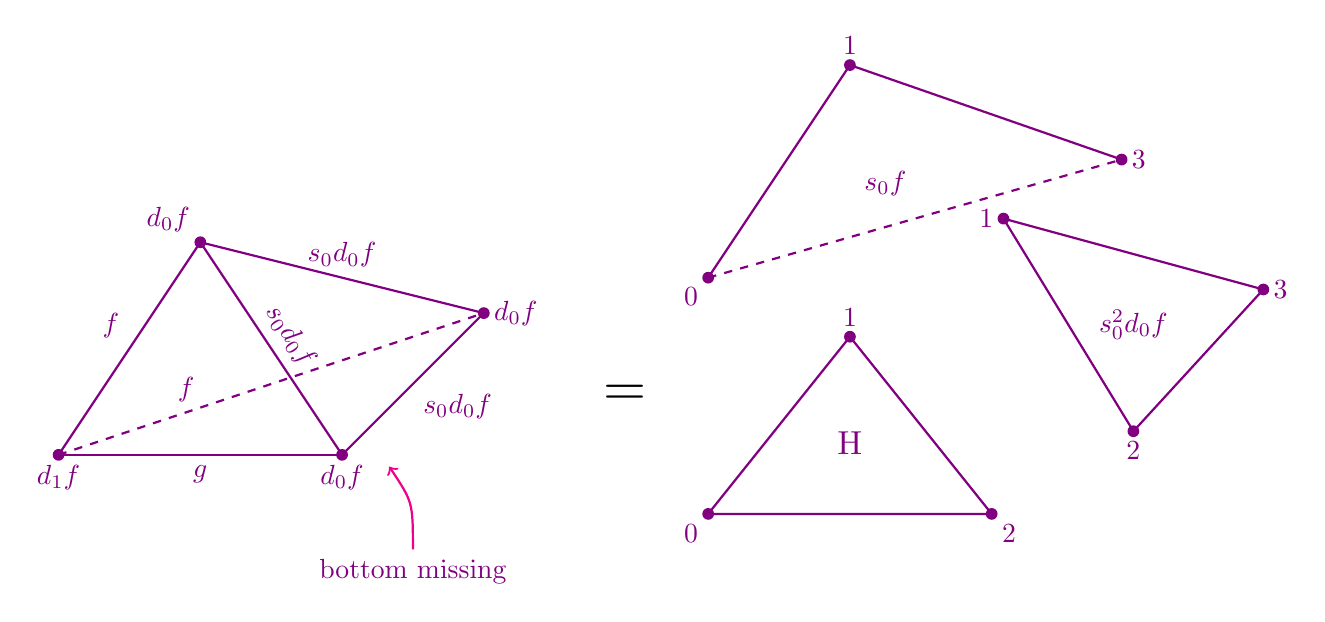
\begin{tikzpicture}[
    scale=1.5,
    every node/.style={text=violet}, % Set default text color to match drawing
    thick,
    color=violet, % Set line color
    dot/.style={circle, fill=violet, inner sep=1.5pt, outer sep=0pt} % Vertex style
]

    % --- LEFT FIGURE (Composite) ---
    
    % Coordinates
    \coordinate (A) at (0,0);       % Bottom Left
    \coordinate (B) at (1.2, 1.8);  % Top
    \coordinate (C) at (2.4, 0);    % Bottom Middle
    \coordinate (D) at (3.6, 1.2);  % Right

    % Edges with labels
    \draw (A) -- node[above left] {$f$} (B);
    \draw (A) -- node[below] {$g$} (C);
    \draw (B) -- node[sloped, above] {$s_0 d_0 f$} (C);
    \draw (B) -- node[above] {$s_0 d_0 f$} (D);
    \draw (C) -- node[below right] {$s_0 d_0 f$} (D);
    
    % Dashed diagonal
    \draw[dashed] (A) -- node[above, pos=0.3] {$f$} (D);

    % Vertices
    \node[dot] at (A) {};
    \node[dot] at (B) {};
    \node[dot] at (C) {};
    \node[dot] at (D) {};

    % Vertex Labels
    \node[below] at (A) {$d_1 f$};
    \node[above left] at (B) {$d_0 f$};
    \node[below] at (C) {$d_0 f$};
    \node[right] at (D) {$d_0 f$};

    % Pink Annotation
    \draw[->, magenta, thick] (3.0, -0.8) node[below] {bottom missing} .. controls (3.0, -0.4) .. (2.8, -0.1);


    % --- EQUALS SIGN ---
    \node[scale=2, text=black] at (4.8, 0.5) {=};


    % --- RIGHT FIGURE (Decomposed) ---

    % 1. Top Triangle (Label: s_0 f)
    \begin{scope}[shift={(5.5, 1.5)}]
        \coordinate (T0) at (0, 0);
        \coordinate (T1) at (1.2, 1.8);
        \coordinate (T3) at (3.5, 1.0); % Stretched to match drawing

        \draw (T0) -- (T1) -- (T3);
        \draw[dashed] (T0) -- (T3);

        \node[dot] at (T0) {};
        \node[dot] at (T1) {};
        \node[dot] at (T3) {};

        \node[below left] at (T0) {0};
        \node[above] at (T1) {1};
        \node[right] at (T3) {3};
        
        % Center Label
        \node at (1.5, 0.8) {$s_0 f$};
    \end{scope}

    % 2. Bottom Left Triangle (Label: H)
    \begin{scope}[shift={(5.5, -0.5)}]
        \coordinate (H0) at (0,0);
        \coordinate (H1) at (1.2, 1.5);
        \coordinate (H2) at (2.4, 0);

        \draw (H0) -- (H1) -- (H2) -- cycle;

        \node[dot] at (H0) {};
        \node[dot] at (H1) {};
        \node[dot] at (H2) {};

        \node[below left] at (H0) {0};
        \node[above] at (H1) {1};
        \node[below right] at (H2) {2};

        % Center Label
        \node[scale=1.2] at (1.2, 0.6) {H};
    \end{scope}

    % 3. Bottom Right Triangle (Label: s_0^2 d_0 f)
    \begin{scope}[shift={(8.0, 0.2)}]
        \coordinate (R1) at (0, 1.8);
        \coordinate (R2) at (1.1, 0);
        \coordinate (R3) at (2.2, 1.2);

        \draw (R1) -- (R2) -- (R3) -- cycle;

        \node[dot] at (R1) {};
        \node[dot] at (R2) {};
        \node[dot] at (R3) {};

        \node[left] at (R1) {1};
        \node[below] at (R2) {2};
        \node[right] at (R3) {3};

        % Center Label
        \node at (1.1, 0.9) {$s_0^2 d_0 f$};
    \end{scope}

\end{tikzpicture}


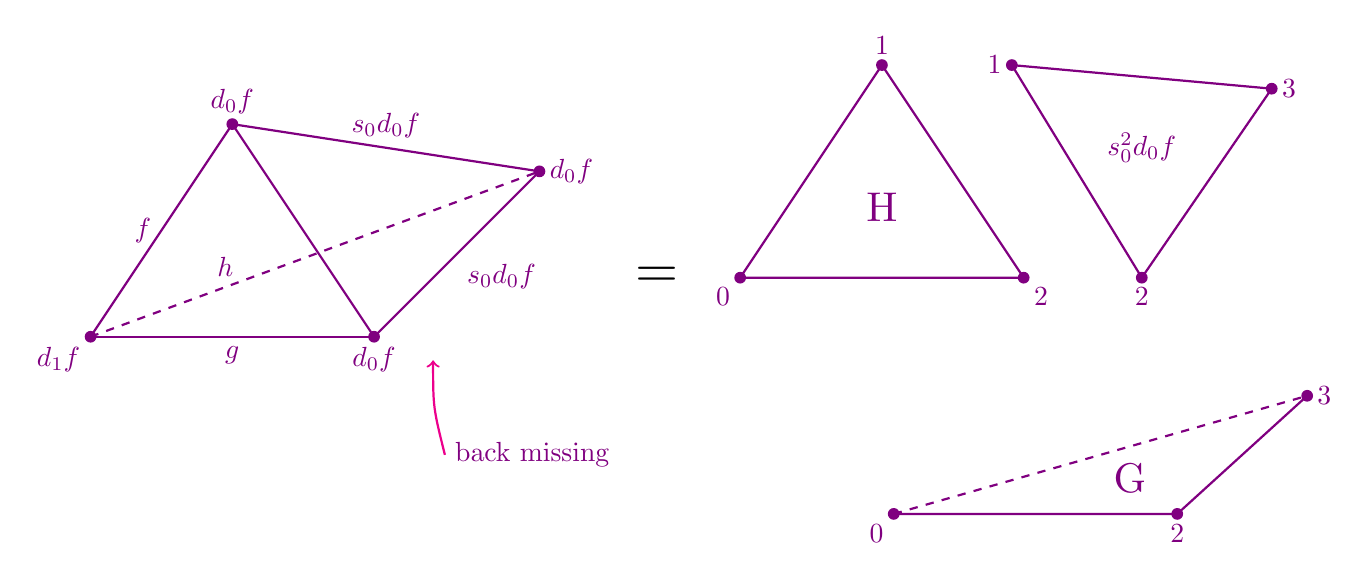
\begin{tikzpicture}[
    scale=1.5,
    thick,
    color=violet, % Main color matching the ink
    every node/.style={text=violet},
    dot/.style={circle, fill=violet, inner sep=1.5pt, outer sep=0pt}
]

    % --- LEFT FIGURE (Composite) ---
    
    % Define coordinates
    \coordinate (L_BL) at (0,0);       % Bottom Left (d_1 f)
    \coordinate (L_Top) at (1.2, 1.8); % Top (d_0 f)
    \coordinate (L_BM) at (2.4, 0);    % Bottom Middle (d_0 f)
    \coordinate (L_R) at (3.8, 1.4);   % Right (d_0 f)

    % Draw solid edges
    \draw (L_BL) -- node[left] {$f$} (L_Top);
    \draw (L_BL) -- node[below] {$g$} (L_BM);
    \draw (L_Top) -- (L_BM); % Middle vertical-ish line
    \draw (L_Top) -- node[above] {$s_0 d_0 f$} (L_R);
    \draw (L_BM) -- node[below right] {$s_0 d_0 f$} (L_R);
    
    % Draw dashed edge (h)
    \draw[dashed] (L_BL) -- node[above, pos=0.3] {$h$} (L_R);

    % Draw Vertices
    \node[dot] at (L_BL) {};
    \node[dot] at (L_Top) {};
    \node[dot] at (L_BM) {};
    \node[dot] at (L_R) {};

    % Vertex Labels
    \node[below left] at (L_BL) {$d_1 f$};
    \node[above] at (L_Top) {$d_0 f$};
    \node[below] at (L_BM) {$d_0 f$};
    \node[right] at (L_R) {$d_0 f$};

    % Pink Annotation "back missing"
    \draw[->, magenta, thick] (3.0, -1.0) node[right] {back missing} .. controls (2.9, -0.6) .. (2.9, -0.2);


    % --- EQUALS SIGN ---
    \node[scale=2, text=black] at (4.8, 0.5) {=};


    % --- RIGHT FIGURE (Decomposed) ---

    % 1. Triangle H (Middle Left)
    \begin{scope}[shift={(5.5, 0.5)}]
        \coordinate (H0) at (0,0);
        \coordinate (H1) at (1.2, 1.8);
        \coordinate (H2) at (2.4, 0);

        \draw (H0) -- (H1) -- (H2) -- cycle;

        \node[dot] at (H0) {};
        \node[dot] at (H1) {};
        \node[dot] at (H2) {};

        \node[below left] at (H0) {0};
        \node[above] at (H1) {1};
        \node[below right] at (H2) {2};

        \node[scale=1.5] at (1.2, 0.6) {H};
    \end{scope}

    % 2. Triangle s_0^2 d_0 f (Top Right)
    \begin{scope}[shift={(7.8, 0.5)}]
        \coordinate (T1) at (0, 1.8);
        \coordinate (T2) at (1.1, 0);
        \coordinate (T3) at (2.2, 1.6);

        \draw (T1) -- (T2) -- (T3) -- cycle;

        \node[dot] at (T1) {};
        \node[dot] at (T2) {};
        \node[dot] at (T3) {};

        \node[left] at (T1) {1};
        \node[below] at (T2) {2};
        \node[right] at (T3) {3};

        \node at (1.1, 1.1) {$s_0^2 d_0 f$};
    \end{scope}

    % 3. Triangle G (Bottom Right)
    \begin{scope}[shift={(6.8, -1.5)}]
        \coordinate (G0) at (0, 0);
        \coordinate (G2) at (2.4, 0);
        \coordinate (G3) at (3.5, 1.0);

        \draw (G0) -- (G2) -- (G3);
        \draw[dashed] (G0) -- (G3);

        \node[dot] at (G0) {};
        \node[dot] at (G2) {};
        \node[dot] at (G3) {};

        \node[below left] at (G0) {0};
        \node[below] at (G2) {2};
        \node[right] at (G3) {3};

        \node[scale=1.5] at (2.0, 0.3) {G};
    \end{scope}

\end{tikzpicture}

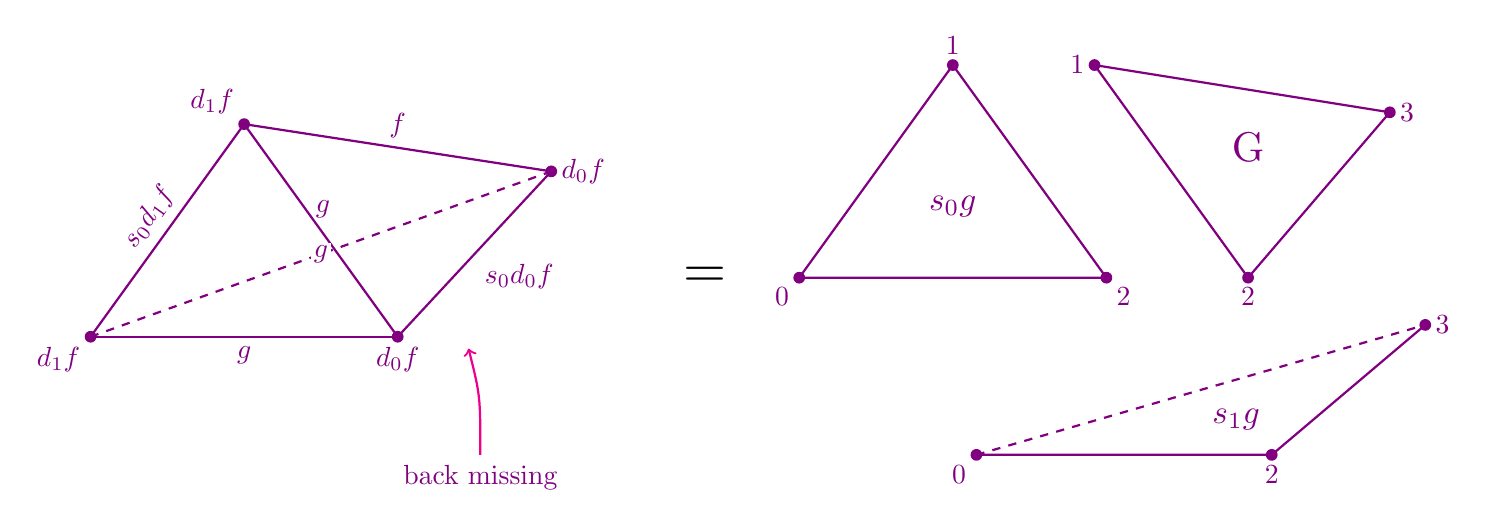
\begin{tikzpicture}[
    scale=1.5,
    thick,
    color=violet, % Match ink color
    every node/.style={text=violet},
    dot/.style={circle, fill=violet, inner sep=1.5pt, outer sep=0pt}
]

    % --- LEFT FIGURE (Composite Shape) ---
    
    % Coordinates
    \coordinate (A) at (0,0);       % Bottom Left
    \coordinate (B) at (1.3, 1.8);  % Top
    \coordinate (C) at (2.6, 0);    % Bottom Middle
    \coordinate (D) at (3.9, 1.4);  % Far Right

    % Solid Edges
    \draw (A) -- node[sloped, above] {$s_0 d_1 f$} (B);
    \draw (A) -- node[below] {$g$} (C);
    \draw (B) -- node[right, pos=0.4] {$g$} (C);
    \draw (B) -- node[above] {$f$} (D);
    \draw (C) -- node[below right] {$s_0 d_0 f$} (D);
    
    % Dashed Edge (diagonal)
    \draw[dashed] (A) -- node[fill=white, inner sep=1pt] {$g$} (D);

    % Vertices (Dots)
    \node[dot] at (A) {};
    \node[dot] at (B) {};
    \node[dot] at (C) {};
    \node[dot] at (D) {};

    % Vertex Labels
    \node[below left] at (A) {$d_1 f$};
    \node[above left] at (B) {$d_1 f$};
    \node[below] at (C) {$d_0 f$};
    \node[right] at (D) {$d_0 f$};

    % Pink Annotation
    \draw[->, magenta, thick] (3.3, -1.0) node[below] {back missing} .. controls (3.3, -0.5) .. (3.2, -0.1);


    % --- EQUALS SIGN ---
    \node[scale=2, text=black] at (5.2, 0.5) {=};


    % --- RIGHT FIGURE (Decomposed Triangles) ---

    % 1. Triangle s_0 g (Middle Left)
    \begin{scope}[shift={(6.0, 0.5)}]
        \coordinate (T1_0) at (0,0);
        \coordinate (T1_1) at (1.3, 1.8);
        \coordinate (T1_2) at (2.6, 0);

        \draw (T1_0) -- (T1_1) -- (T1_2) -- cycle;

        \node[dot] at (T1_0) {};
        \node[dot] at (T1_1) {};
        \node[dot] at (T1_2) {};

        \node[below left] at (T1_0) {0};
        \node[above] at (T1_1) {1};
        \node[below right] at (T1_2) {2};

        \node[scale=1.2] at (1.3, 0.6) {$s_0 g$};
    \end{scope}

    % 2. Triangle G (Top Right)
    \begin{scope}[shift={(8.5, 0.5)}]
        \coordinate (T2_1) at (0, 1.8);    % Top Left
        \coordinate (T2_2) at (1.3, 0);    % Bottom Middle
        \coordinate (T2_3) at (2.5, 1.4);  % Right

        \draw (T2_1) -- (T2_2) -- (T2_3) -- cycle;

        \node[dot] at (T2_1) {};
        \node[dot] at (T2_2) {};
        \node[dot] at (T2_3) {};

        \node[left] at (T2_1) {1};
        \node[below] at (T2_2) {2};
        \node[right] at (T2_3) {3};

        \node[scale=1.5] at (1.3, 1.1) {G};
    \end{scope}

    % 3. Triangle s_1 g (Bottom Right)
    \begin{scope}[shift={(7.5, -1.5)}]
        \coordinate (T3_0) at (0, 0.5);
        \coordinate (T3_2) at (2.5, 0.5);
        \coordinate (T3_3) at (3.8, 1.6);

        \draw (T3_0) -- (T3_2) -- (T3_3);
        \draw[dashed] (T3_0) -- (T3_3);

        \node[dot] at (T3_0) {};
        \node[dot] at (T3_2) {};
        \node[dot] at (T3_3) {};

        \node[below left] at (T3_0) {0};
        \node[below] at (T3_2) {2};
        \node[right] at (T3_3) {3};

        \node[scale=1.2] at (2.2, 0.8) {$s_1 g$};
    \end{scope}

\end{tikzpicture}

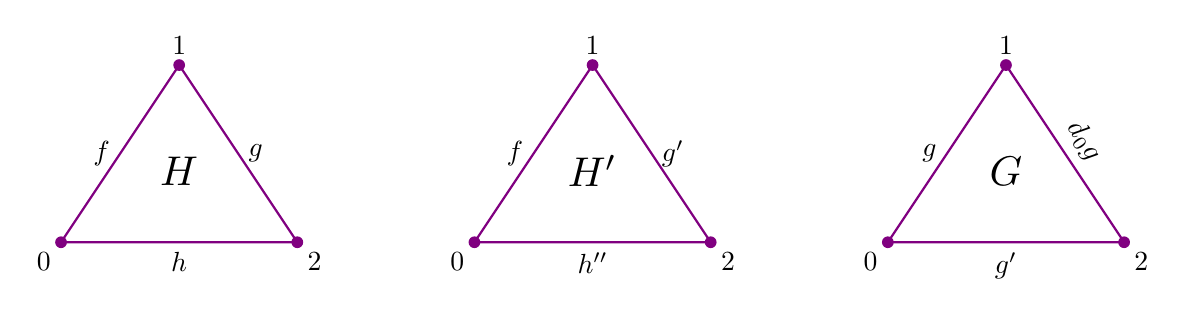
\begin{tikzpicture}[
    scale=1.5,
    thick,
    color=violet, % Match ink color
    every node/.style={text=black},
    dot/.style={circle, fill=violet, inner sep=1.5pt, outer sep=0pt}
]

    % --- Triangle 1 (Left) ---
    \begin{scope}[shift={(0,0)}]
        \coordinate (A1) at (0,0);
        \coordinate (B1) at (1,1.5);
        \coordinate (C1) at (2,0);

        \draw (A1) -- node[left] {$f$} (B1)
              -- node[right] {$g$} (C1)
              -- node[below] {$h$} (A1);

        \node[dot] at (A1) {}; \node[below left] at (A1) {0};
        \node[dot] at (B1) {}; \node[above]      at (B1) {1};
        \node[dot] at (C1) {}; \node[below right] at (C1) {2};

        \node[scale=1.5] at (1, 0.6) {$H$};
    \end{scope}

    % --- Triangle 2 (Middle) ---
    \begin{scope}[shift={(3.5,0)}]
        \coordinate (A2) at (0,0);
        \coordinate (B2) at (1,1.5);
        \coordinate (C2) at (2,0);

        \draw (A2) -- node[left] {$f$} (B2)
              -- node[right] {$g'$} (C2)
              -- node[below] {$h''$} (A2); % Label appears to be h double-prime

        \node[dot] at (A2) {}; \node[below left] at (A2) {0};
        \node[dot] at (B2) {}; \node[above]      at (B2) {1};
        \node[dot] at (C2) {}; \node[below right] at (C2) {2};

        \node[scale=1.5] at (1, 0.6) {$H'$};
    \end{scope}

    % --- Triangle 3 (Right) ---
    \begin{scope}[shift={(7,0)}]
        \coordinate (A3) at (0,0);
        \coordinate (B3) at (1,1.5);
        \coordinate (C3) at (2,0);

        \draw (A3) -- node[left] {$g$} (B3)
              -- node[sloped, above] {$d_0 g$} (C3)
              -- node[below] {$g'$} (A3);

        \node[dot] at (A3) {}; \node[below left] at (A3) {0};
        \node[dot] at (B3) {}; \node[above]      at (B3) {1};
        \node[dot] at (C3) {}; \node[below right] at (C3) {2};

        \node[scale=1.5] at (1, 0.6) {$G$};
    \end{scope}

\end{tikzpicture}


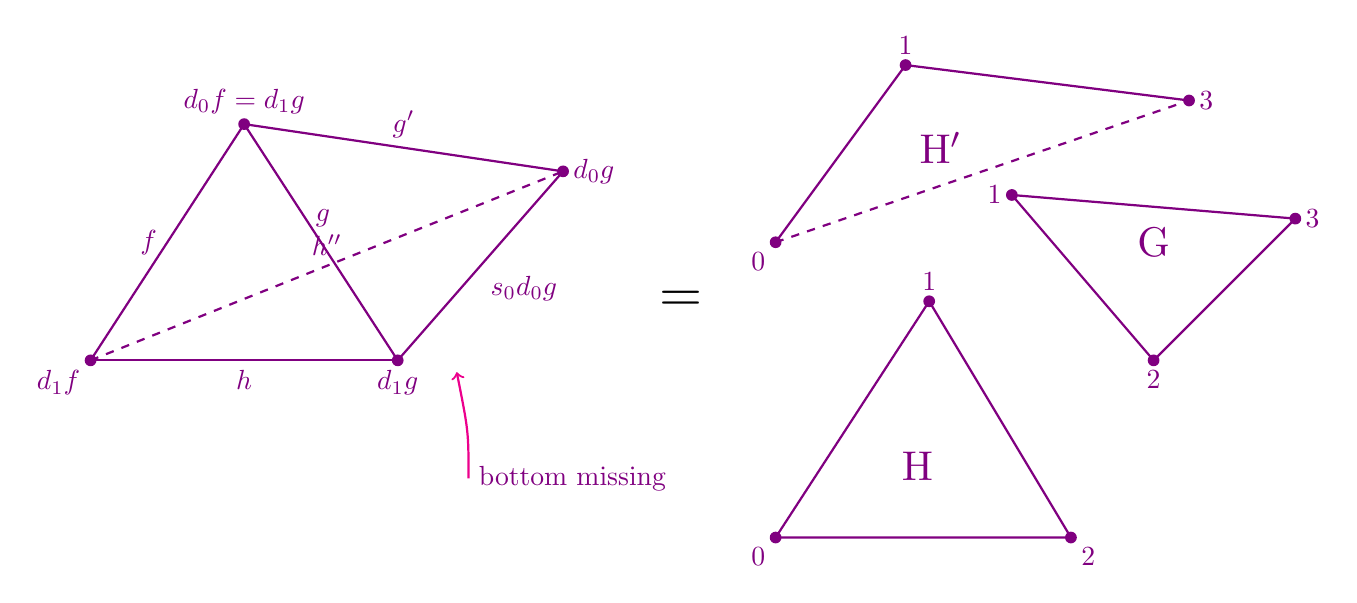
\begin{tikzpicture}[
    scale=1.5,
    thick,
    color=violet, % Match ink color
    every node/.style={text=violet},
    dot/.style={circle, fill=violet, inner sep=1.5pt, outer sep=0pt}
]

    % --- LEFT FIGURE (The Complex) ---
    
    % Coordinates
    \coordinate (L0) at (0,0);       % Bottom Left (d_1 f)
    \coordinate (L1) at (1.3, 2.0);  % Top (d_0 f = d_1 g)
    \coordinate (L2) at (2.6, 0);    % Bottom Middle (d_1 g)
    \coordinate (L3) at (4.0, 1.6);  % Right (d_0 g)

    % Draw solid edges
    \draw (L0) -- node[left] {$f$} (L1);
    \draw (L0) -- node[below] {$h$} (L2);
    \draw (L1) -- node[right, pos=0.4] {$g$} (L2);
    \draw (L1) -- node[above] {$g'$} (L3);
    \draw (L2) -- node[below right] {$s_0 d_0 g$} (L3);
    
    % Draw dashed edge
    \draw[dashed] (L0) -- node[above, pos=0.5] {$h''$} (L3);

    % Draw Vertices
    \node[dot] at (L0) {};
    \node[dot] at (L1) {};
    \node[dot] at (L2) {};
    \node[dot] at (L3) {};

    % Vertex Labels
    \node[below left] at (L0) {$d_1 f$};
    \node[above] at (L1) {$d_0 f = d_1 g$};
    \node[below] at (L2) {$d_1 g$};
    \node[right] at (L3) {$d_0 g$};

    % Pink Annotation "bottom missing"
    % Note: The text looks like "bottom missing" pointing to the empty face 0-2-3
    \draw[->, magenta, thick] (3.2, -1.0) node[right] {bottom missing} .. controls (3.2, -0.6) .. (3.1, -0.1);


    % --- EQUALS SIGN ---
    \node[scale=2, text=black] at (5.0, 0.5) {=};


    % --- RIGHT FIGURE (Decomposed Triangles) ---

    % 1. Triangle H' (Top Left)
    \begin{scope}[shift={(5.8, 1.0)}]
        \coordinate (H1_0) at (0, 0);
        \coordinate (H1_1) at (1.1, 1.5);
        \coordinate (H1_3) at (3.5, 1.2); % Stretched to match dashed line geometry

        \draw (H1_0) -- (H1_1) -- (H1_3);
        \draw[dashed] (H1_0) -- (H1_3);

        \node[dot] at (H1_0) {};
        \node[dot] at (H1_1) {};
        \node[dot] at (H1_3) {};

        \node[below left] at (H1_0) {0};
        \node[above] at (H1_1) {1};
        \node[right] at (H1_3) {3};

        \node[scale=1.5] at (1.4, 0.8) {H$'$};
    \end{scope}

    % 2. Triangle H (Bottom Left)
    \begin{scope}[shift={(5.8, -1.5)}]
        \coordinate (H0) at (0,0);
        \coordinate (H1) at (1.3, 2.0);
        \coordinate (H2) at (2.5, 0);

        \draw (H0) -- (H1) -- (H2) -- cycle;

        \node[dot] at (H0) {};
        \node[dot] at (H1) {};
        \node[dot] at (H2) {};

        \node[below left] at (H0) {0};
        \node[above] at (H1) {1};
        \node[below right] at (H2) {2};

        \node[scale=1.5] at (1.2, 0.6) {H};
    \end{scope}

    % 3. Triangle G (Right)
    \begin{scope}[shift={(7.8, 0.0)}]
        \coordinate (G1) at (0, 1.4);
        \coordinate (G2) at (1.2, 0);
        \coordinate (G3) at (2.4, 1.2);

        \draw (G1) -- (G2) -- (G3) -- cycle;

        \node[dot] at (G1) {};
        \node[dot] at (G2) {};
        \node[dot] at (G3) {};

        \node[left] at (G1) {1};
        \node[below] at (G2) {2};
        \node[right] at (G3) {3};

        \node[scale=1.5] at (1.2, 1.0) {G};
    \end{scope}

\end{tikzpicture}

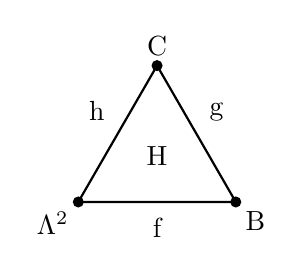
\begin{tikzpicture}

    % Define the coordinates for an equilateral triangle
    % A at origin, B at 4 units right, C at 60 degrees (polar coordinates)
    \coordinate (A) at (0,0);
    \coordinate (B) at (2,0);
    \coordinate (C) at (60:2);

    % Draw the triangle and label the sides
    % 'midway' is implicit for nodes on paths
    % sloped creates a label aligned with the line, but standard text is usually preferred for basic geometry
    \draw[thick] (A) -- node[below=2pt] {f} (B) 
                     -- node[above right=1pt] {g} (C) 
                     -- node[above left=1pt] {h} cycle;

    % Draw the vertices: Small filled circles and text labels
    % Circle radius is set to 2pt
    \fill (A) circle (2pt) node[below left] {$\Lambda^2$};
    \fill (B) circle (2pt) node[below right] {B};
    \fill (C) circle (2pt) node[above] {C};

    % Label the center "H"
    % Uses the barycentric coordinate system to find the exact geometric center
    \node at (barycentric cs:A=1,B=1,C=1) {H};

\end{tikzpicture}

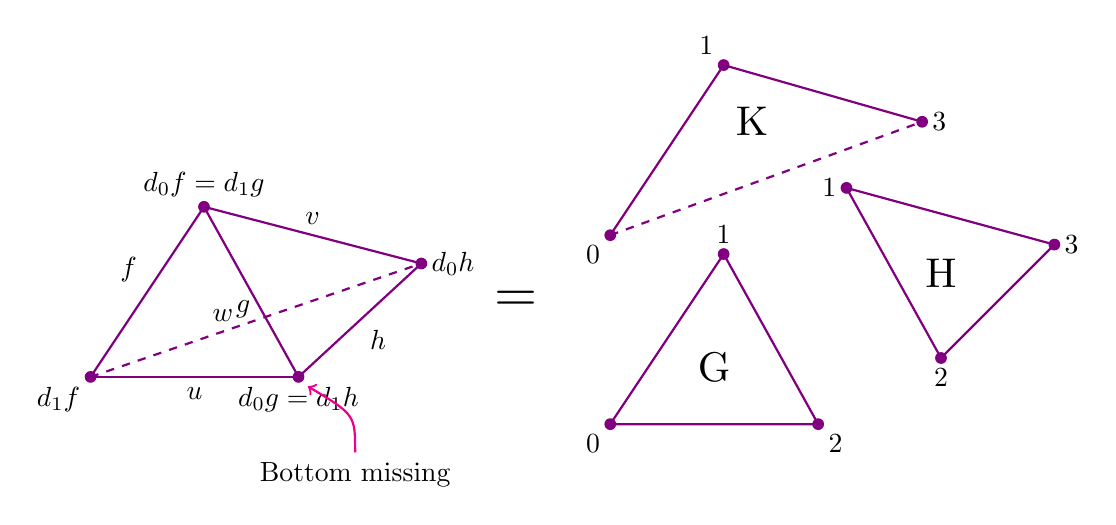
\begin{tikzpicture}[
    scale=1.2, 
    every node/.style={text=black}, 
    thick, 
    color=violet,
    dot/.style={circle, fill=violet, inner sep=1.5pt} % Style for the small filled circles
]

    % --- LEFT FIGURE (The Complex) ---
    
    % Define coordinates
    \coordinate (L0) at (0,0);       % Bottom Left (0)
    \coordinate (L1) at (1.2, 1.8);  % Top (1)
    \coordinate (L2) at (2.2, 0);    % Bottom Middle (2)
    \coordinate (L3) at (3.5, 1.2);  % Right (3)

    % Draw solid lines
    \draw (L0) -- node[above left] {$f$} (L1);
    \draw (L0) -- node[below] {$u$} (L2);
    \draw (L1) -- node[left, pos=0.6] {$g$} (L2);
    \draw (L1) -- node[above] {$v$} (L3);
    \draw (L2) -- node[below right] {$h$} (L3);
    
    % Draw dashed line
    \draw[dashed, thick] (L0) -- node[above, pos=0.4] {$w$} (L3);

    % Draw Vertices (dots)
    \node[dot] at (L0) {};
    \node[dot] at (L1) {};
    \node[dot] at (L2) {};
    \node[dot] at (L3) {};

    % Vertex Labels (Math expressions based on handwriting)
    \node[below left] at (L0) {$d_1 f$};
    \node[above] at (L1) {$d_0 f = d_1 g$};
    \node[below] at (L2) {$d_0 g = d_1 h$};
    \node[right] at (L3) {$d_0 h$};

    % Pink annotation "Bottom missing"
    \draw[->, magenta, thick] (2.8, -0.8) node[below] {Bottom missing} .. controls (2.8, -0.4) .. (2.3, -0.1);


    % --- EQUALS SIGN ---
    \node[scale=2] at (4.5, 0.8) {=};


    % --- RIGHT FIGURE (Decomposed Triangles) ---

    % -- Triangle G (Bottom Left) --
    \begin{scope}[shift={(5.5, -0.5)}]
        \coordinate (G0) at (0,0);
        \coordinate (G1) at (1.2, 1.8);
        \coordinate (G2) at (2.2, 0);
        
        \draw (G0) -- (G1) -- (G2) -- cycle;
        
        \node[dot] at (G0) {};
        \node[dot] at (G1) {};
        \node[dot] at (G2) {};
        
        \node[below left] at (G0) {0};
        \node[above] at (G1) {1};
        \node[below right] at (G2) {2};
        
        \node[scale=1.5] at (1.1, 0.6) {G};
    \end{scope}

    % -- Triangle H (Bottom Right) --
    \begin{scope}[shift={(8, 0.2)}]
        \coordinate (H1) at (0, 1.8);    % Relative 1
        \coordinate (H2) at (1.0, 0);    % Relative 2
        \coordinate (H3) at (2.2, 1.2);  % Relative 3
        
        \draw (H1) -- (H2) -- (H3) -- cycle;
        
        \node[dot] at (H1) {};
        \node[dot] at (H2) {};
        \node[dot] at (H3) {};
        
        \node[left] at (H1) {1};
        \node[below] at (H2) {2};
        \node[right] at (H3) {3};
        
        \node[scale=1.5] at (1.0, 0.9) {H};
    \end{scope}

    % -- Triangle K (Top) --
    \begin{scope}[shift={(5.5, 1.5)}]
        \coordinate (K0) at (0, 0);
        \coordinate (K1) at (1.2, 1.8);
        \coordinate (K3) at (3.3, 1.2); % Stretched out like the drawing
        
        \draw (K0) -- (K1) -- (K3);
        \draw[dashed] (K0) -- (K3);
        
        \node[dot] at (K0) {};
        \node[dot] at (K1) {};
        \node[dot] at (K3) {};
        
        \node[below left] at (K0) {0};
        \node[above left] at (K1) {1};
        \node[right] at (K3) {3};
        
        \node[scale=1.5] at (1.5, 1.2) {K};
    \end{scope}

\end{tikzpicture}

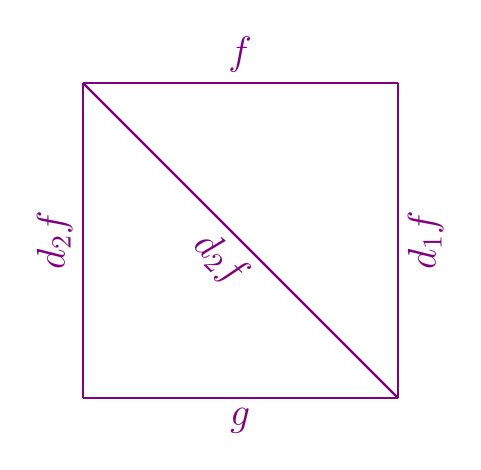
\begin{tikzpicture}[
    scale=2, 
    thick, 
    color=violet, 
    every node/.style={text=violet, font=\Large}
]

    % Define Coordinates
    \coordinate (TL) at (0,2); % Top Left
    \coordinate (TR) at (2,2); % Top Right
    \coordinate (BL) at (0,0); % Bottom Left
    \coordinate (BR) at (2,0); % Bottom Right

    % Draw Square Edges
    \draw (TL) -- node[above] {$f$} (TR);
    \draw (BL) -- node[below] {$g$} (BR);
    
    % Draw Vertical Edges with rotated labels
    % 'rotate=90' aligns the text vertically reading upwards
    \draw (BL) -- node[above, rotate=90] {$d_2 f$} (TL);
    \draw (BR) -- node[below, rotate=90] {$d_1 f$} (TR);

    % Draw Diagonal
    % 'sloped' aligns text with the line
    \draw (TL) -- node[sloped, below] {$d_2 f$} (BR);

\end{tikzpicture}